\documentclass{article}
\usepackage{amssymb}
\usepackage{amsmath}
\usepackage{physics}
\usepackage{graphicx}
\usepackage{subfig}
\usepackage{tikz}
\graphicspath{ {./images/} }
\setcounter{tocdepth}{3}
  
\newcommand{\keywords}[1]{\par\addvspace\baselineskip
\noindent\keywordname\enspace\ignorespaces#1}

\DeclareMathOperator{\EX}{\mathbb{E}}

\begin{document}

\mainmatter


\title{An application of methods from Deep Learning and Statistical Physics to combinatorial optimization problems}

\titlerunning{DL and NQS for IP problems}


\author{Semyon Sinchenko\inst{1} \and Dmitry Bazhanov\inst{1,2,3}}

\authorrunning{Lecture Notes in Computer Science}


\institute{Moscow Aviation Institute,\\
Volokolamskoe shosse, 4, Moscow, 125993, Russian Federation\\
\and
Faculty of Physics, Moscow State University,\\
GSP-1, Leninskie Gory, Moscow, 119991, Russian Federation\\
\and
Institution of Russian Academy of Sciences,\\
Dorodnicyn Computing Centre of RAS, Vavilov St. 40, Moscow,  119333, Russian Federation
}

\toctitle{Lecture Notes in Computer Science}
\maketitle


\begin{abstract}
The present work aims to apply the methods from statistical physics and deep learning to solve the MaxCut problem. In recent time there appeared some advanced techniques for solving the many-body problems in quantum physics that based on artificial deep neural networks. And from the State of the Art we know that the quantum many-body problems can be shown as problems of combinatorial optimization. For the MaxCut problem we describe the corresponding quantum system and with help of deep learning approach we found found the ground state of that system. Next we go back to corresponding MaxCut problems and seen that solution from quantum physics is the solution of the original MaxCut problem. We test our approach on the two graphs. For graph with 60 vertices and 885 edges we get the cut with size 0.99\% of known maximal cut. For graph with 100 vertices and 2475 edges we get the cut with size 0.98\% of maximal cut.
\keywords{neural networks, deep learning, quantum physics, integer programming, maxcut}
\end{abstract}

\section{Introduction}
\subsection{The MaxCut problem}
The MaxCut problem is well-studied problem in combinatorial optimization and integer programming. The problem defined as follow:

Given the Graph $G = (V, V)$ where $E$ is the edges set and $V$ is the vertices set. For simplify the problem we will analyse only unweighted and undirected graphs but at the end we will talk about the generalization of our ansatz. The MaxCut problem is to find the subsets of vertices $V_1$ and $V_2$ such that the number of edges that incident to vertices from different sets are maximal:
$$\sum_{i,j \in E} (1 - x_ix_j) \to Max$$
where $x_i = 1$ if the vertex is from $V_1$ and $x_i = -1$ if the vertex is from $V_2$.

We also define here the \textit{performance} $p$ for given algorithm $H$ that give us the cut of size $C$:
$$p_H = \frac{C}{MaxCutSize}$$

\subsection{Known approaches}
The MaxCut-problem is NP-hard and exact solution that can be found by the branch and bound method is unfeasible in case of medium and large graphs. There are some approximation algorithms for solving the MaxCut problem but the best of them give the solution only about $\sim 0.9$ \textit{performance}\cite{MaxCutClassic}.

\section{Energy minimisation approach}
\subsection{Quantum many-body problem}
Searching of the wave function $\Psi$ of the many-body systems is one of the most important but one of the hardest problems in quantum physics. The wave function contains the whole information of the state of any quantum system (atoms, particles, etc.) and known the wave function dynamic allow to predict the state of the system at each moment. Formally the wave-function $\Psi$ is the complex-valued function and it's square modulus is the probability of get state $\ket{\psi}$ (here $\ket{x}$ is the vector in the Hilbert space) as result of measurements. The wave function of the system can be found analytically as a solution of the Schroedinger equation: $$i\hbar\frac{d}{dt}\ket{\Psi(t)} = \hat{H}\ket{\Psi(t)}$$
where $\hat{H}$ is the Hamiltonian operator that corresponds to the kinetic and potential energy of the system. However the amount of information that is needed to fully encode the many-body system growths exponentially in the number of particles.

The necessity of the computing integrals or sums (in discrete case) on all Hilbert space fail the direct approaches to solving the many-body problems. One of the popular solution is Quantum Monte Carlo methods that use variations of the Monte-Carlo method to estimate integrals over configuration space\cite{VMC} in polynomial time. Another popular approach names Matrix product State that is the generalization of numeric renormalization-group procedure to quantum lattice and more general Tensor Networks approach. But there are some examples of physical systems where described approaches fail\cite{VMCfail}.

\subsection{The couple of MaxCut and quantum Hamiltonian}
From the State of the Art\cite{MaxCutHam} known some attempts to solve the quantum many-body problem. 

Let's imagine for the given graph $G$ the quantum system that comprises $|V|$ quantum particles with quantum spins $s = \{+1, -1\}$ and define the quantum Hamiltonian on such graph:
$$\hat{H} = \frac{1}{2}\sum_{i,j \in E}A_{ij}(1 - \sigma^z_i\sigma^z_j)$$
where $A$ is the adjacency matrix of our graph and $\sigma^z$ is the Pauli matrix:
$$\sigma^z  = \begin{pmatrix}
	1& 0\\
	0& -1
\end{pmatrix}$$

The ground state or the state with minimal energy for that quantum system. If we define the $V_1$ and $V_2$ vertices subsets as $V_1 = \{x_i: s_i = 1\}$ and $V_2 = \{x_i: s_i = -1\}$ then the ground state of our quantum system give us the solution of MaxCut problem. The reverse is also true: if we solve the MaxCut problem we also found the ground state of the corresponding quantum system.

This approach actively developing in the area of Quantum Information Theory and the area of Quantum Algorithms\cite{QAOA}\cite{QA} and show the excellent results on experimental quantum computers for small graphs.


\subsection{Neural Quantum States}
The new approach to solve the quantum many-body problem presented in 2017\cite{CarleoScience} is based on the Neural Networks. We define the Neural Network with one hidden layer as function $F(\bf{x})$ that fully described by the matrix of weights $\bf{W}$, vector of biases $\bf{b}$ and the activation functions $\sigma$: $$F(\bf{x}) = \sigma(\bf{b} + \bf{W}\vdot{\bf{x}})$$By the Cybenko universal approximation theorem\cite{Cybenko} any function $[0, 1]^n\to{[0, 1]}$ can be approximated by neural network with one hidden layer with any precision. There is the generalization of that theorem to Complex Plane\cite{ComplexCybenko}. In such a manner theoretically for each real quantum system there is the Neural Network with weights $\bf{W}$ and biases $\bf{b}$ such that the output of that network approximate the $\Psi$ function of that system.

We can define the deep neural network (in our case that was a simple Feed-Forward Neural Network -- FFNN) that give us the oracle. That oracle can say the probability of any state of our system. With that oracle we can apply the MCMC-methods\cite{MCMC} and get the samples from the distribution defined by our $\Psi$-function.

From physical principles we know that each physical system tend to the state with minimal energy (ground state). Based on that knowledge we can define the energy-minimization procedure:
\begin{itemize}
\item With oracle get samples from distribution defined by FFNN
\item Estimate the energy of samples and the expectation of energy
\item Estimate the Gradient of energy [THERE WE NEED TO COPY-PASTE FORMULAS FROM CARLEO LECTURES WHERE HE ESTIMATE THE GRADIENT]
\item Update weights and biases of FFNN by usage of Gradient-Descent method
\end{itemize}

\subsection{Comparison with simulated Annealing}
Principally the nearest approach to our NQS-based ansatz is the method that called simulated Annealing. 

\begin{tikzpicture}
\node (sample) [startstop] {New permuted sample}
\node (energy) [process, right of=sample] {Calculate energy}
\nide (accept) [process, below of=energy] {Accept with $p \sim Gibbs(E_{old}, E_{permuted}, T$}
\end{tikzpicture}


\section{Experiments}
We take two graphs from the Biq-Mac collection\cite{BiqMac}: graph with name \textbf{g05\_60.0} (60 vertices, 884 edges) and graph with name \textbf{g05\_100.0} (100 vertices, 2474 edges):


\begin{figure}
\centering
\subfloat[60-vertex graph]{{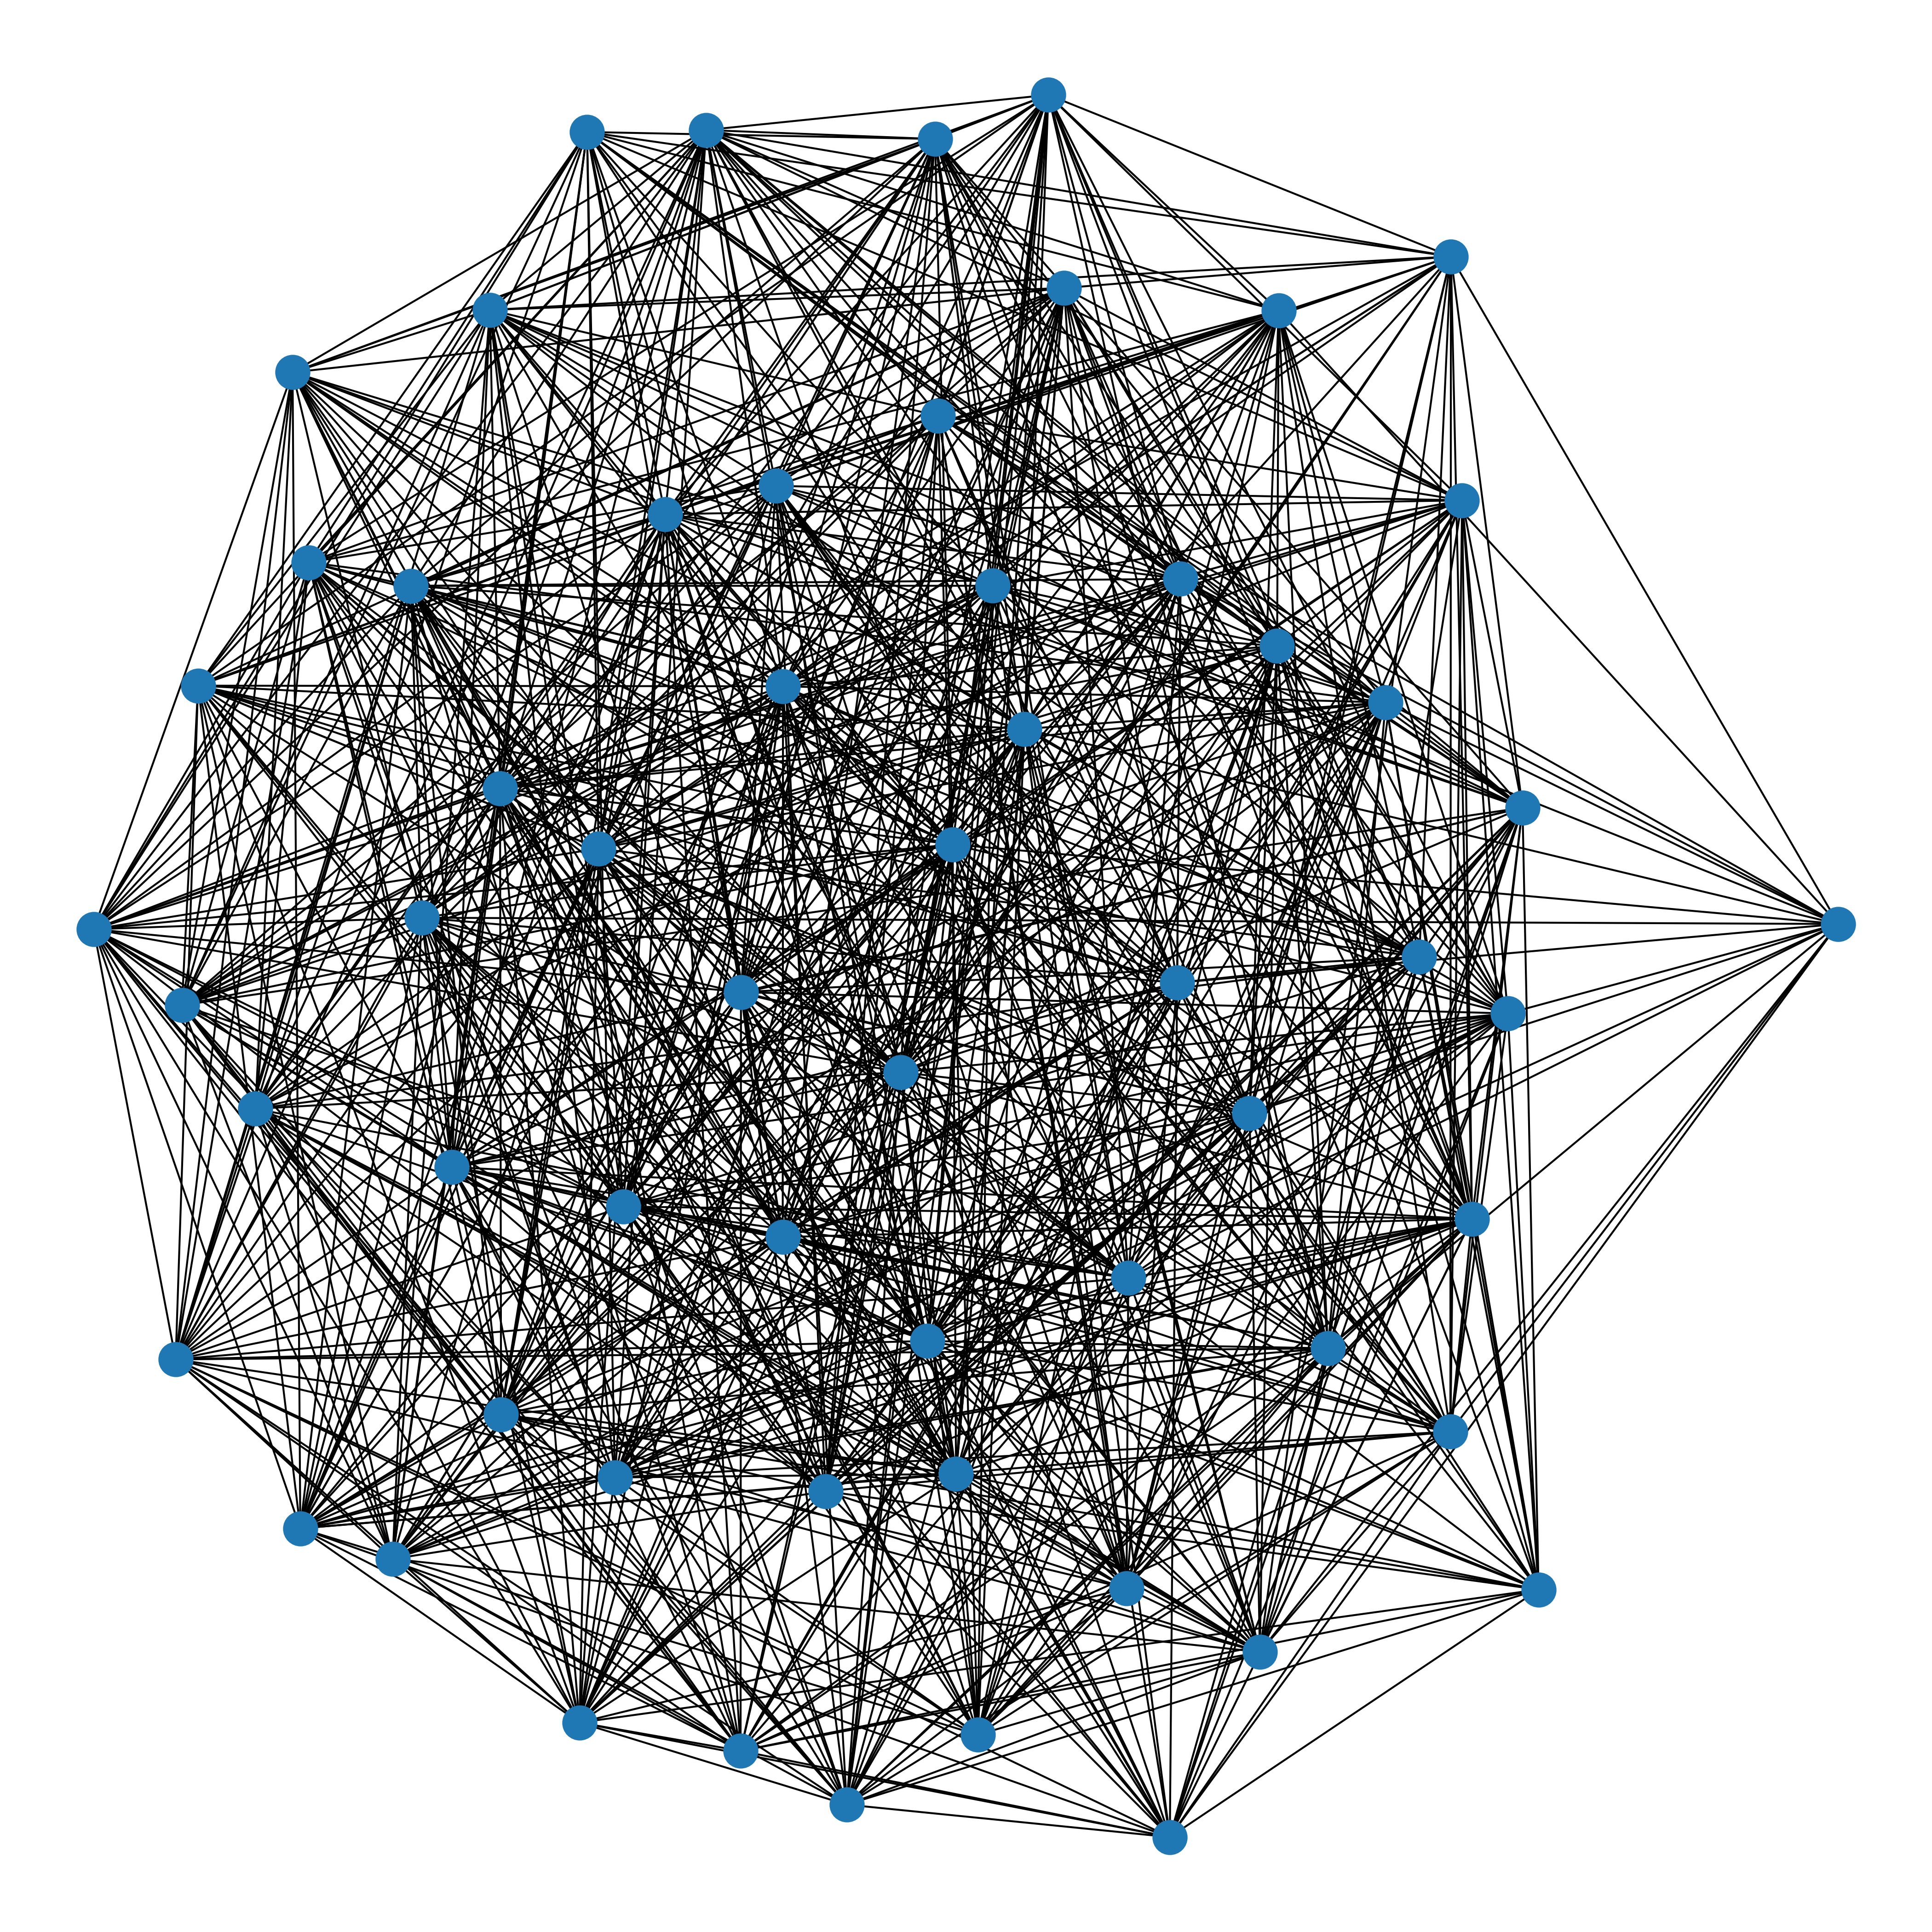
\includegraphics[scale=0.1]{60vertexG}}}
\qquad
\subfloat[100-vertex graph]{{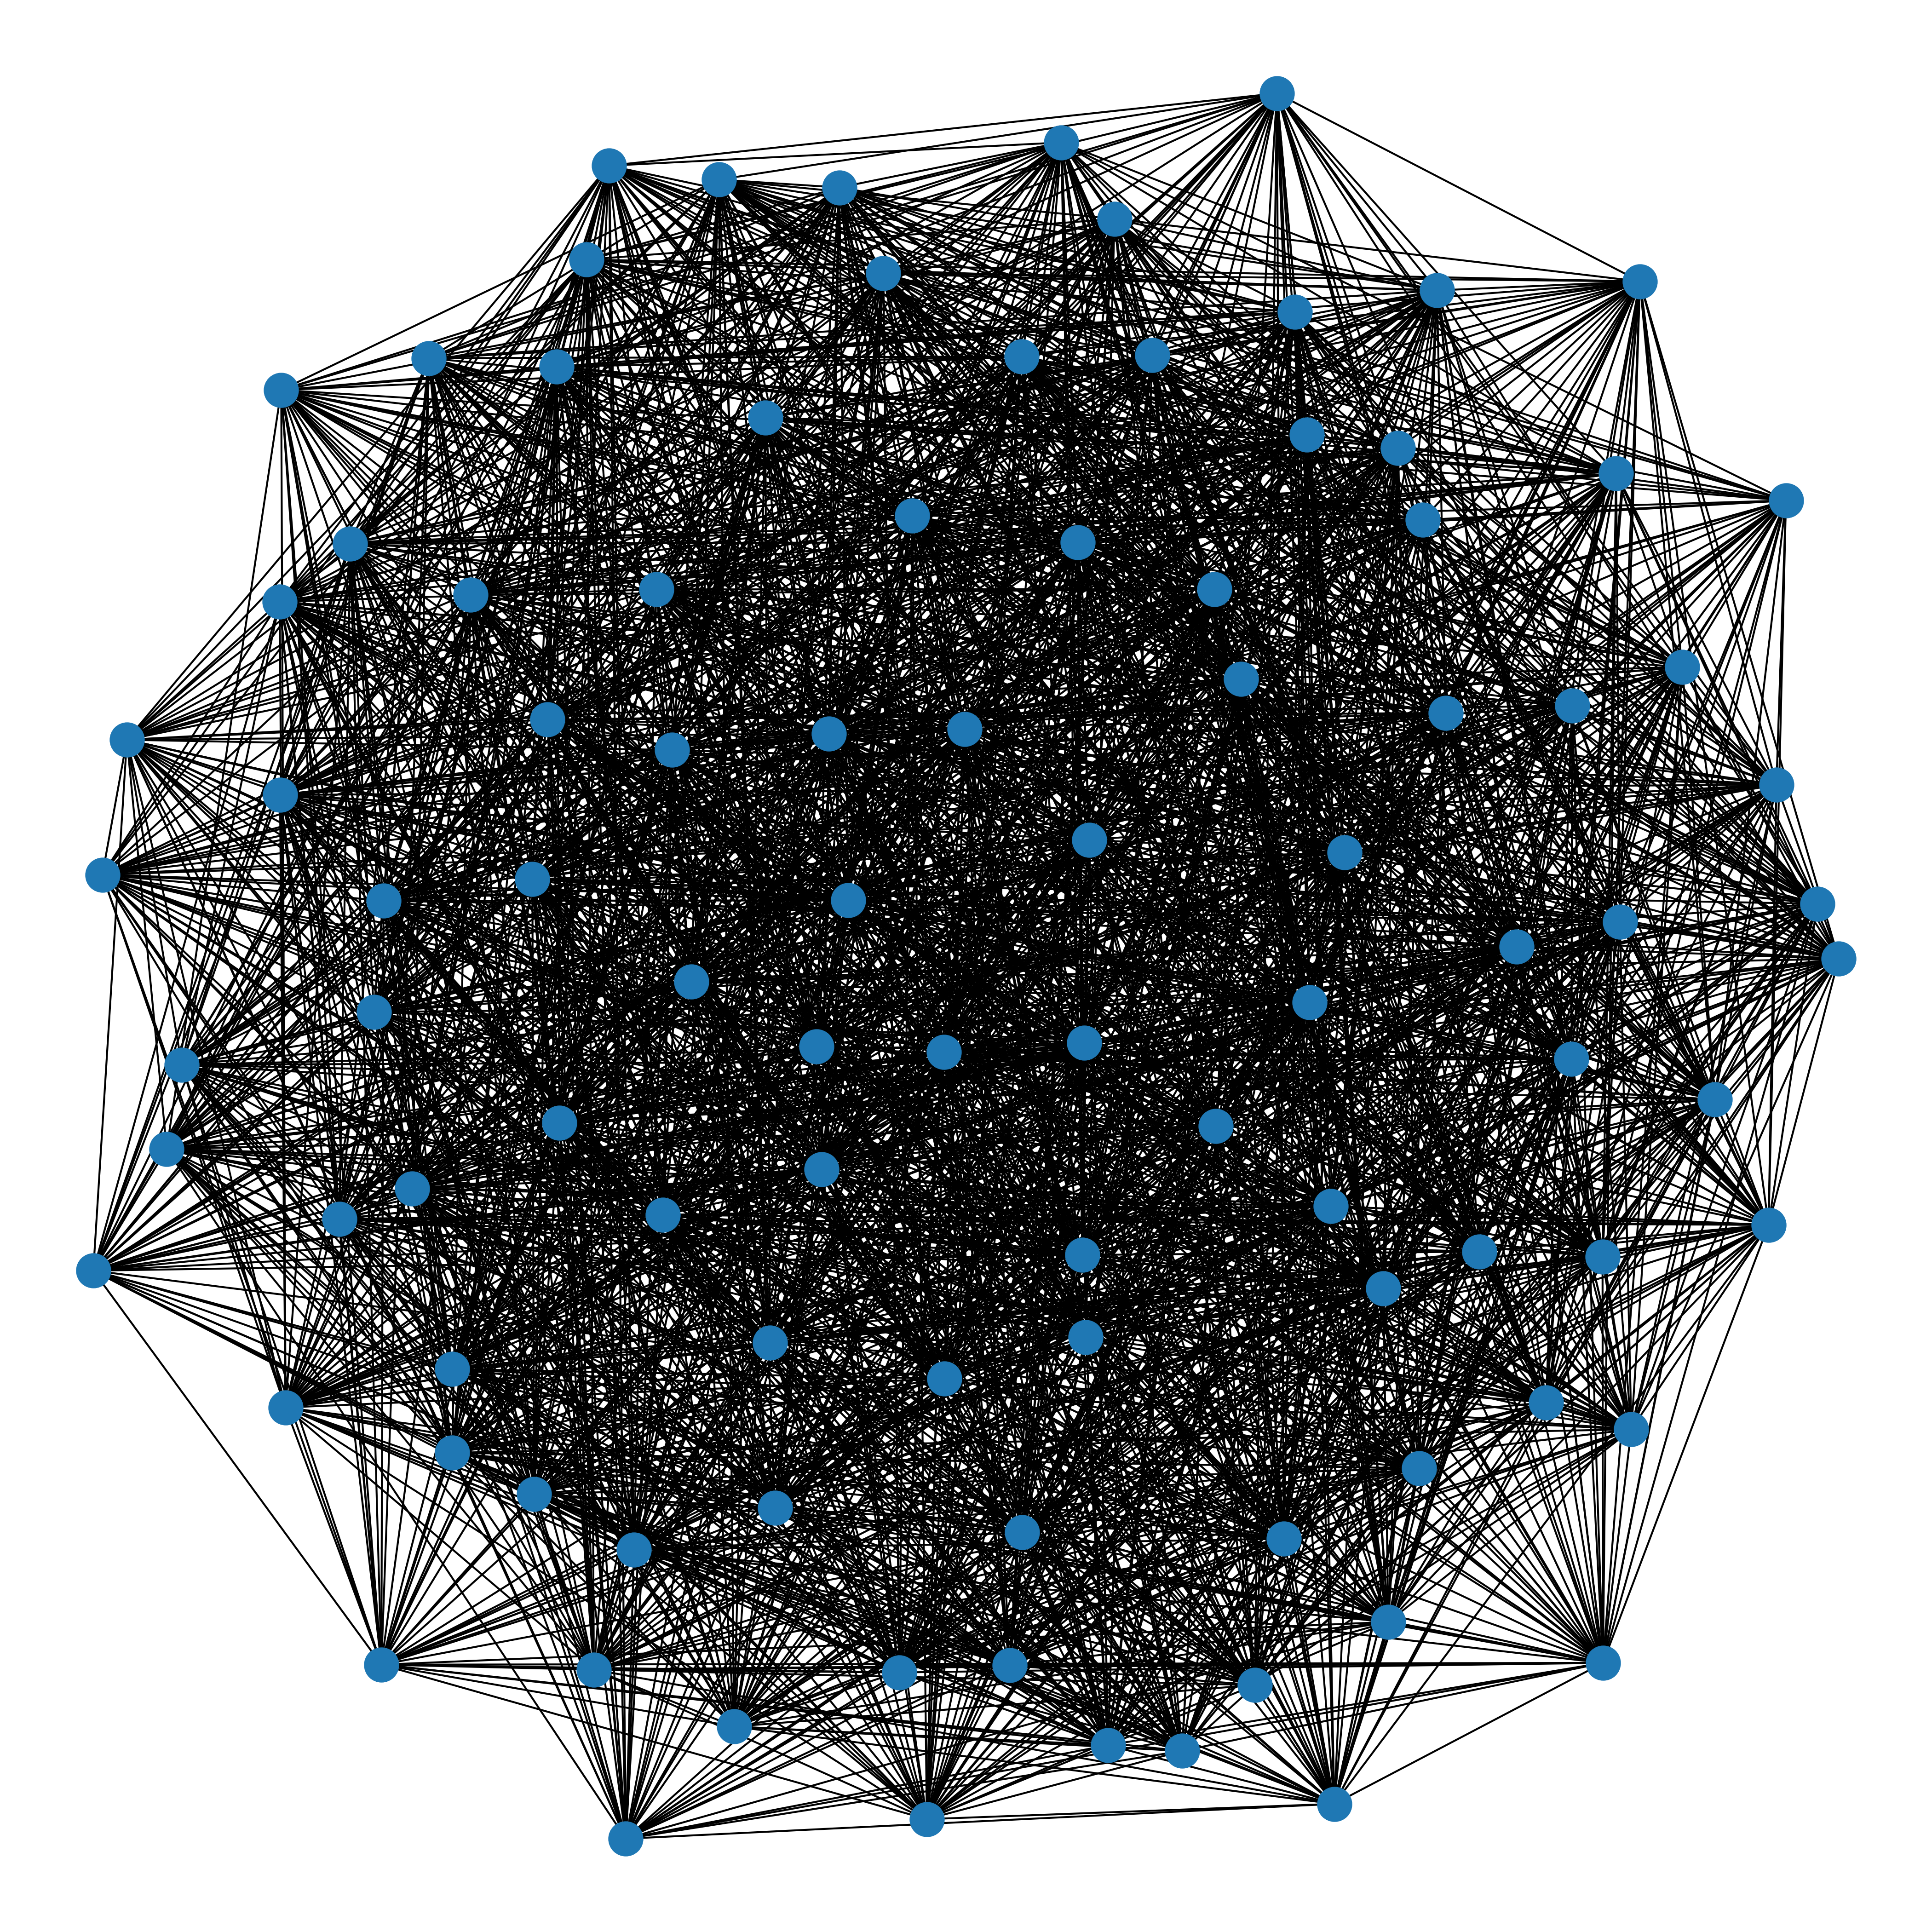
\includegraphics[scale=0.1]{100vertexG}}}
\caption{Used graphs}
\end{figure}

For each of that graph we define the corresponding quantum Hamiltonian and apply the Neural Quantum State approach to found the ground state energy.

Next we get 2000 samples from our oracle that defined by our Neural Network. For each sample we calculate the cut size.

For apply NQS procedure we used the NetKet library\cite{netket}

\subsection{Network Architecture for 60-vertex graph}
For small graph we used the following structure:
\begin{itemize}
\item Fully-Connected layer: input shape 60, output shape 30
\item Fully-Connected layer: input shape 30, output shape 20
\item Fully-Connected layer: input shape 20, output shape 10
\item LnCosh layer
\item Sum layer
\end{itemize}


Learning Hyper Parameters:
\begin{center}
\begin{tabular}[center]{| l | r |}
\hline
Optimizer & Nesterov momentum ($lr=0.008, \beta = 0.9$) \\ \hline
Samples at each step & 6000 \\ \hline
Discarded samples at each step (first N) & 3000 \\ \hline
Learning epochs & 400 \\
\hline
\end{tabular}
\end{center}


\subsection{Network Architecture for 100-vertex graph}
For small graph we used the following structure:
\begin{itemize}
\item Fully-Connected layer: input shape 60, output shape 40
\item Fully-Connected layer: input shape 40, output shape 30
\item Fully-Connected layer: input shape 30, output shape 10
\item LnCosh layer
\item Sum layer
\end{itemize}

Learning Hyper Parameters:
\begin{center}
\begin{tabular}[center]{| l | r |}
\hline
Optimizer & Nesterov momentum ($lr=0.008, \beta = 0.9$) \\ \hline
Samples at each step & 10000 \\ \hline
Discarded samples at each step (first N) & 5000 \\ \hline
Learning epochs & 800 \\
\hline
\end{tabular}
\end{center}

\section{Results}
\subsection{60-vertex graph}
Learning curve:
\begin{figure}
\centering
\includegraphics[scale=0.3]{resultPlot60}
\caption{Learning curve (left), energy variance (center), acceptance rate (right)}
\end{figure}

We can see that mean energy for samples converged to known optimal solution of MaxCut problem. Also we can see that variety of states converged to zero and in most cases we get the same state for each sample.

Next we get 2000 samples from final oracle:
\begin{figure}
\centering
\includegraphics[scale=0.4]{samples60}
\caption{Cut size for 2000 samples}
\end{figure}

We can see that the \textit{performance} is about 0.99\%.

\subsection{100-vertex graph}
Learning curve:
\begin{figure}
\centering
\includegraphics[scale=0.3]{resultPlot100}
\caption{Learning curve (left), energy variance (center), acceptance rate (right)}
\end{figure}

We can see that mean energy for samples converged to known optimal solution of MaxCut problem. Also we can see that variety of states converged to zero and in most cases we get the same state for each sample.

Next we get 2000 samples from final oracle:
\begin{figure}
\centering
\includegraphics[scale=0.4]{samples100}
\caption{Cut size for 2000 samples}
\end{figure}

We can see that the \textit{performance} is about 0.97\%.

\begin{thebibliography}{20}
\bibitem{MaxCutClassic} Bian, Y., Gronskiy, A., & Buhmann, J. M. (2016). Information-theoretic analysis of MaxCut algorithms. In 2016 Information Theory and Applications Workshop (ITA) (pp. 1–5).
\bibitem{VMC} Metropolis, N., Rosenbluth, A. W., Rosenbluth, M. N., Teller, A. H., & Teller, E. (1953). Equation of state calculations by fast computing machines. Journal of Chemical Physics, 21(6), 1087–1092.
\bibitem{MPS} White, S. R. (1992). Density matrix formulation for quantum renormalization groups. Physical Review Letters, 69(19), 2863–2866.
\bibitem{VMCfail} Troyer, M., & Wiese, U.-J. (2005). Computational complexity and fundamental limitations to fermionic quantum Monte Carlo simulations. Physical Review Letters, 94(17), 170201.
\bibitem{MaxCutHam} Barahona, F., Grötschel, M., Jünger, M., & Reinelt, G. (1988). An application of combinatorial optimization to statistical physics and circuit layout design. Operations Research, 36(3), 493–513.
\bibitem{QAOA} Crooks, G. E. (2018). Performance of the Quantum Approximate Optimization Algorithm on the Maximum Cut Problem. ArXiv Preprint ArXiv:1811.08419.
\bibitem{QA} Glen Bigan Mbeng, Rosario Fazio, Giuseppe Santoro (2019). Quantum Annealing: a journey through Digitalization, Control, and hybrid Quantum Variational schemes. ArXiv Preprint ArXiv:1906.08948
\bibitem{CarleoScience} Carleo, Giuseppe, and Matthias Troyer. "Solving the quantum many-body problem with artificial neural networks." Science 355.6325 (2017): 602-606.
\bibitem{Cybenko} Cybenko, George. "Approximations by superpositions of a sigmoidal function." Mathematics of Control, Signals and Systems 2 (1989): 183-192.
\bibitem{ComplexCybenko} Kim, Taehwan, and Tülay Adalı. "Approximation by fully complex multilayer perceptrons." Neural computation 15.7 (2003): 1641-1666.
\bibitem{MCMC} Gilks, W. R., Richardson, S., & Spiegelhalter, D. (1997). Markov Chain Monte Carlo in Practice. Technometrics, 39(3), 338–338.
\bibitem{BiqMac} Wiegele, A. (2007). Biq Mac Library—A collection of Max-Cut and quadratic 0-1 programming instances of medium size. Preprint.
\bibitem{netket} Carleo, Giuseppe, et al. (2019). NetKet: A Machine Learning Toolkit for Many-Body Quantum Systems. ArXiv Preprint ArXiv:1904.00031 

\end{thebibliography}
\end{document}